                                                                                                                                                                                                                                                                                                                                                                                                                                                                                                                                                                                                                                                                                                                                                                                                                                                                                                                                                                                                                                                                                                                                                                                                                                                                                                                                                                                                                                                                                                                                                                                                                                                                                                                                                                                                                                                                                                                                                                                                                                                                                                                                                                                                                                                                                                                                                                                                                                                                                                                                                                                                                                                                                                                                                                                                                                                                                                                                                                                                                                                                                                                                                                                                                                                                                                                                                                                                                                                                                                                                                                                                                                                                                                                                                                                                                                                                                                                                                                                                                                                                                                                                                                                                                                                                                                                                                                                                                                                                                                                                                                                                                                                                                                                                                                                                                                                                        \documentclass[english]{tktltiki}
\usepackage[pdftex]{graphicx}
\usepackage{subfigure}
\usepackage{url}
\usepackage{amsmath}

\begin{document}
%\doublespacing
%\singlespacing
\onehalfspacing

\title{IMSE, A content based image retrieval system}
\author{Sayantan Hore}
\date{\today}

\maketitle

\numberofpagesinformation{\numberofpages\ pages + \numberofappendixpages\ appendices}
\classification{\protect{\ \\
A.1 [Introductory and Survey],\\
I.7.m [Document and text processing]}}

\keywords{layout, summary, list of references}

\begin{abstract}

Content based image retrieval systems are out there for a few years now. We present a system, IMSE, here which searches out images using Gaussian Process Upper Confidence Bound algorithm. This algorithm has performed better in comparison to random search and plain exploration. We present a comparison of how the algorithm performs on CPU as well as GPU. We also evaluate the user experience and with the search interface.

\end{abstract}

\mytableofcontents




\section{Introduction}


Content based image retrieval systems have been proven to be better fits in retrieval performance. Text or tag based matching systems rely only on texts. Therefore the images themselves are secondary in the search procedure. The user sees the image and selects one by the objects and color the image represents. The combination of those objects and colors should actually be searched for instead of tags. Tags hardly represent an entire image. An image portraying a cloudy afternoon can be tagged as "Sad", based on the mood and understanding of the person creating the tags. Another images of the same genre, tagged by different persons, might miss the tag. If a user is in search for "Sad" images and finds one with the tag, selects it. The other "Sad" image would not appear in the search results as it lacks the tag. Had features and content of the image been searched for, this situation could be avoided.

IMSE is just another content based image retrieval system, using Gaussian Process Upper Confidence Bound (GP-UCB) as a retrieval algorithm. We are using MIRFLICKR 25000 image set for testing. As this produces a huge kernel, GP-UCB is slow on CPU. We have written a GPU version of the algorithm and made a comparative study of running time over CPU and GPU. The system is written in Python (and Django for the web interface). Any system has to have a pleasing and assisting user interface. As our system is targeted towards web users, we cared for having a decent web interface, written in Twitter Bootstrap (v3.0) framework, jQuery (v1.11.1), CSS and javascript. We have followed Human Computer Interaction guidelines for user interaction.

In subsequent section, we will present the theoretical background of Reinforcement Learning, Gaussian Process, Upper Confidence Bound, Image Retrieval, GPU implementation details, user experience and performance measures.


\section{The need for content based retrieval in detail}

...

\subsection{Shortcomings of traditional image search}
%\enlargethispage{5mm}

...

\subsection{Why content based retrieval is better}


...


\subsection{Approaches}

...

%\pagebreak

\section{Theoretical background}

...


\subsection{Reinforcement Learning}

...

\subsection{Regression Problems}

Regression problems are supervised learning problems where we have multiple random variables. At least one of those variables are dependant on a subset of the rest. Lets' assume that we have to predict rainfall prediction in a city for the coming monsoon based on average summer temperature. We first take a dataset consisting of year by year rainfall and average summer temperature recorded over the past few years. We denote the temperature by $x$ and rainfall by $y$. Clearly $x$ is an independent random variable and $y$ is dependent on $x$. We take a set $S = \{x_i, y_i\}$ for the past years. The goal here is to learn the relation between $x$ and $y$. We will apply the relation on unknown $x$ values to get the corresponding $y$ values. Here relation basically means a mathematical function.

In its simplest form the function could be a linear one like,

\begin{equation}
f(x_i) = \theta_1 x_i + \theta_0
\end{equation}


But often in real life scenarios we have more than one independent variables. Besides temperature we can have amount of $CO_2$ emission, amount of deforestation (in square kilometres) and so forth. Therefore in these cases instead of having a single $x_i$ we have a vector $\mathbf{x}_i = \{x_{i1}, x_{i2}, x_{i3}, ..., x_{im}\}$. We rewrite equation 1 as,

\begin{equation}
f(\mathbf{x}_i) = \sum_{j=1}^m \theta_j x_{ij} + \theta_0
\end{equation}

It is not possible to match each and every $y_i$ because of the randomness of the data. We try to go as close as possible so that $f(x)$ can represent the pattern of the output. The closeness is measured by \textit{least square} method. The goal is to minimize the distance between $y_i$ and $f(x_i)$ over the entire dataset. Say $d^2_i$ represents the squared distance between $y_i$ and $f(x_i)$.

\begin{eqnarray}
d^2_i = [y_i - f(\mathbf{x}_i)]^2
\end{eqnarray}

Let $d^2$ denote the summation of all $d^2_i$,

\begin{eqnarray}
d^2 = \sum_i[y_i - f(\mathbf{x}_i)]^2 \nonumber\\
d^2 = \sum_i[y_i - \sum_{j=1}^m \theta_j x_{ij} - \theta_0]^2 \nonumber\\
d^2 = \sum_i[y_i - \theta_1x_{i1} - \theta_2x_{i2} - \theta_3x_{i3} - ... - \theta_mx_{im} - \theta_0]^2
\end{eqnarray}

To obtain minimum $d^2$ we take partial derivative with respect to each $\theta_i$ and set those to zero. Therefore we get a set of partial differential equations as follows,

\begin{eqnarray}
\frac{\partial}{\partial{\theta_0}}(d^2) = -2\sum_i[y_i - \theta_1x_{i1} - \theta_2x_{i2} - \theta_3x_{i3} - ... - \theta_mx_{im} - \theta_0] = 0\nonumber \\
\frac{\partial}{\partial{\theta_1}}(d^2) = -2\sum_i[y_i - \theta_1x_{i1} - \theta_2x_{i2} - \theta_3x_{i3} - ... - \theta_mx_{im} - \theta_0]x_{i1} = 0\nonumber \\
\frac{\partial}{\partial{\theta_2}}(d^2) = -2\sum_i[y_i - \theta_1x_{i1} - \theta_2x_{i2} - \theta_3x_{i3} - ... - \theta_mx_{im} - \theta_0]x_{i2} = 0\nonumber \\
\vdots \nonumber \\
\frac{\partial}{\partial{\theta_m}}(d^2) = -2\sum_i[y_i - \theta_1x_{i1} - \theta_2x_{i2} - \theta_3x_{i3} - ... - \theta_mx_{im} - \theta_0]x_{im} = 0
\end{eqnarray}

Assuming we have n observed data points, We can write this set of equations as,

\begin{eqnarray}
\theta_0 n + \theta_1 \sum_{i=1}^n x_{i1} + \theta_2 \sum_{i=1}^n x_{i2} + ... + \theta_m \sum_{i=1}^n x_{im} = \sum_{i=1}^n y_i \nonumber \\
\theta_0 \sum_{i=1}^n x_{i1} + \theta_1 \sum_{i=1}^n x_{i1}^2 + \theta_2 \sum_{i=1}^n x_{i1} x_{i2} +  ... + \theta_m \sum_{i=1}^n x_{i1} x_{im} = \sum_{i=1}^n y_i x_1 \nonumber \\
\theta_0 \sum_{i=1}^n x_{i2} + \theta_1 \sum_{i=1}^n x_{i1} x_{i2} + \theta_1 \sum_{i=1}^n x_{i2}^2 + ... + \theta_m \sum_{i=1}^n x_{i2} x_{im} = \sum_{i=1}^n y_i x_2 \nonumber \\
\vdots \nonumber \\
\theta_0 \sum_{i=1}^n x_{im} + \theta_1 \sum_{i=1}^n x_{i1} x_{im} + \theta_1 \sum_{i=1}^n x_{i2} x_{im} + ... + \theta_m \sum_{i=1}^n x_{im}^2 = \sum_{i=1}^n y_i x_m
\end{eqnarray}

This can be written in matrix form,

$$
\begin{pmatrix}
\sum_{i=1}^n y_i \\
\sum_{i=1}^n y_i x_i \\
\sum_{i=1}^n y_i x_2 \\
\vdots \\
\sum_{i=1}^n y_i x_m
\end{pmatrix}
=%
\begin{pmatrix}
n & \sum_{i=1}^n x_{i1} & \sum_{i=1}^n x_{i2} \hdots \sum_{i=1}^n x_{im} \\
\sum_{i=1}^n x_{i1} & \sum_{i=1}^n x_{i1}^2 & \sum_{i=1}^n x_{i1} x_{i2} \hdots \sum_{i=1}^n x_{i1} x_{im} \\
\sum_{i=1}^n x_{i2} & \sum_{i=1}^n x_{i1} x_{i2} & \sum_{i=1}^n x_{i2}^2 \hdots \sum_{i=1}^n x_{i2} x_{im} \\
\vdots&\vdots \\
\sum_{i=1}^n x_{im} & \sum_{i=1}^n x_{i1} x_{im} & \sum_{i=1}^n x_{i2} x_{im} \hdots \sum_{i=1}^n x_{im}^2 \\
\end{pmatrix}
%
\begin{pmatrix}
\theta_0 \\
\theta_1 \\
\theta_2 \\
\vdots \\
\theta_m
\end{pmatrix}
$$

In simplified notation,

\begin{eqnarray}
\mathbf{Y} = \mathbf{X \theta} \nonumber \\
\mathbf{X^TY} = \mathbf{X^T X \theta} \nonumber \\
\mathbf{\theta} = \mathbf{(X^T X)^{-1} X^T Y}
\end{eqnarray}

We obtained the optimal $\theta$.

\subsection{Gaussian Distribution}

A one dimensional random variable $x$, which Gaussian distribution with mean $\mu$ and variance $\sigma$ has a PDF,

\begin{equation}
p(x) = \frac{1}{\sqrt{2 \pi}\sigma} \exp(\frac{(x - \mu)^2}{2 \sigma^2})
\end{equation}



This is the equation of a bell curve as shown in Figure \ref{fig:gaussian_1d}.

Eqn. 8 can be written as,

\begin{equation}
p(x) \sim \mathcal{N}(\mu, \sigma^2)
\end{equation}

It means, $x$ comes from a Gaussian distribution with mean $\mu$ and variance $\sigma^2$.

Sometimes we have a collection of random variables $\mathbf{x} = \{x_1, x_2, x_3, ..., x_m\}, m \in \mathcal{R}$, where each $x_i, i \in m$ follows Gaussian distribution, we write the PDF over $\mathbf{x}$ as,

\begin{equation}
p(\mathbf{x}) = \frac{1}{\sqrt{(2 \pi)^m |\Sigma|}}exp(-\frac{1}{2}(\mathbf{x} - \mu)^T \Sigma^{-1} (\mathbf{x} - \mu))
\end{equation}

Here $\mu = \{\mu_1, \mu_2, ..., \mu_m\}$ is a mean vector where each $\mu_i$ represents the mean of $x_i$ where $i \in m$. $\Sigma$ is a $mXm$ covariance matrix where any $\Sigma[i, j]$ represents the co-variance between $x_i$ and $x_j$.

Figure \ref{fig:gaussian_2d} shows the plot of a two dimensional Gaussian.

We can write Eqn. 10 as,

\begin{equation}
p(\mathbf{x}) \sim \mathcal{N}(\mathbf{\mu}, \Sigma^2)
\end{equation}

\begin{figure}
\centering
\begin{minipage}{.5\linewidth}
  \centering
  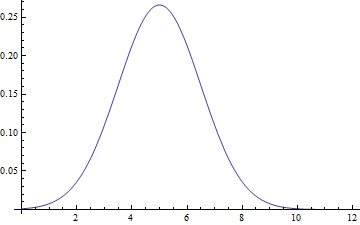
\includegraphics[width=\linewidth]{gp_1d.png}
  \caption{Univariate Gaussian}
  \label{fig:gaussian_1d}
\end{minipage}%
\begin{minipage}{.41\linewidth}
  \centering
  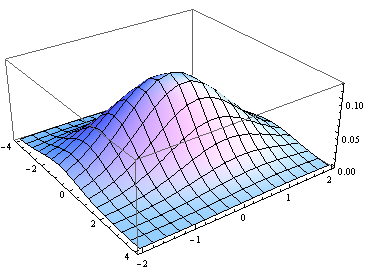
\includegraphics[width=\linewidth]{gp_2d.png}
  \caption{Multivariate Gaussian}
  \label{fig:gaussian_2d}
\end{minipage}

\label{fig:test}
\end{figure}


\subsection{Bayesian Probability Model}

The traditional linear regression method is rigid in terms of learning the parameters. It gives fixed values for parameters for one observed dataset. Therefore for every new observed datapoint, the parameters are bound to change. It would be effective to learn a probability distribution over the parameters rather than fixed values. Having a distribution over parameters gives us space where the parameters can move, which is convenient to understand a stochastic process. Bayesian probability model starts with a prior distribution over parameters and changes the distribution based on observations.

Bayesian probability model is built after \textit{Bayes'} rule. It allows us to start with a prior belief on the data, which is an initial probability distribution associated to the data. Experiments generate evidences, which are used to change the prior belief, i.e. the initial distribution. The new distribution we get after incorporating the evidences is called posterior. The formulation is given below.

\subsubsection{Bayes' Rule}

We start with the expression of Bayes' rule. Say we have two random variables, $x$ and $y$, where $x$ is an independent variable but $y$ depends on $x$. The probability of $x$ is given by $p(x)$, the joint probability of $x$ and $y$ is given by $p(y, x)$. We can break $p(y, x)$ in $p(y|x)p(x)$ or $p(x|y)p(y)$ (Here $p(x|y)$ cannot be written as $p(x)$ if $x$ is conditionally dependant on $y$). Therefore,

\begin{eqnarray}
p(y, x) = p(y|x)p(x) = p(x|y)p(y)\nonumber\\
p(y|x) = \frac{p(x|y)p(y)}{p(x)}
\end{eqnarray}


The term $p(x)$ is marginalized over all possible values of $y$, so we can write $p(x)$ as,

\begin{equation}
p(x) = \sum_i{p(x|y_i)p(y_i)}
\end{equation}


Combining Eqn. 8 and Eqn. 9,

\begin{equation}
p(y|x) = \frac{p(x|y)p(y)}{\sum_i{p(x|y_i)p(y_i)}}
\end{equation}

In case $y$ is a continuous variable,

\begin{equation}
p(y|x) = \frac{p(x|y)p(y)}{\int_y{p(x|y)p(y)dy}}
\end{equation}

We start with the assumption that $y_i$ differs from $f(\mathbf{x}_i)$ because of noise, also Each noise term $\epsilon_i$ follows Gaussian i.i.d. $\mathcal{N}(0, \sigma ^2)$. Therefore the i\textsuperscript{th} can be written as,

\begin{eqnarray}
y_i = f(\mathbf{x}_i) + \epsilon_i \nonumber \\
y_i = \theta ^T \mathbf{x}_i + \epsilon_i && \text{where $\theta, \mathbf{x}_i \in \mathcal{R}^m$}
\end{eqnarray}

The PDF associated with $\epsilon_i$ is,

\begin{equation}
p(\epsilon_i) = \frac{1}{\sqrt{2 \pi} \sigma} exp(-\frac{\epsilon^2}{2 \sigma^2})
\end{equation}


It follows from Eqn. 9 that $(y_i - \theta ^T x_i) \sim \mathcal{N}(0, \sigma^2)$, so by combining Eqn. 9 and Eqn. 10,

\begin{equation}
p(y_i - \theta ^T x_i) = \frac{1}{\sqrt{2 \pi} \sigma} exp(-\frac{(y_i - \theta ^T x_i)^2}{2 \sigma^2})
\end{equation}

From Eqn. 11 we conclude,

\begin{eqnarray}
\begin{split}
&p(y_i - \theta ^T \mathbf{x}_i) \sim \mathcal{N}(0, \sigma^2) \nonumber \\
&p(y_i | \mathbf{x}_i, \theta) \sim \mathcal{N}(\theta^T \mathbf{x}_i, \sigma^2)
\end{split}
\end{eqnarray}

We need to calculate the distribution over $\theta$ based on observed dataset $S = \{\mathbf{x}_i, y_i\}_{i=1}^n$ consisting of $n$ data points. The conditional PDF over $\theta$ given $S$ would be,

\begin{eqnarray}
\begin{split}
p(\theta | S) &= \frac{p(\theta)p(S | \theta)}{p(S)} \nonumber \\
&~\\
p(\theta | S) &= \frac{p(\theta)p(S | \theta)}{\int p(\theta)p(S | \theta)d\theta} \nonumber \\
&~\\
p(\theta | S) &= \frac{p(\theta) \prod_{i=1}^n p(y_i | \mathbf{x}_i, \theta)}{\int p(\theta) \prod_{i=1}^n p(y_i | \mathbf{x}_i, \theta) d\theta}
\end{split}
\end{eqnarray}

We need to predict $y_*$ for the next unobserved data point $S_* = {y_*, x_*}$ for some $x_*$ given $S$ which can be formulated as below,

\begin{equation}
p(y_* | x_*, S) = \int p(y_* | x_*, \theta)p(\theta | S)d \theta
\end{equation}

\subsection{Gaussian Process}

The problem with the multivariate Gaussian distribution is that we are confined to the number of operating variables or the dimension of the input $\mathbf{x_i} \in \mathcal{R}^m$. Therefore to calculate the posterior distribution for $y_*$, we had to go for a two step solution. Firstly we learned a multivariate Gaussian posterior $p(\theta | S)$ over the set of parameters $\theta \in \mathcal{R}^m$ and secondly used it to calculate the posterior over $y_*$.

It would be nice to have a mathematical framework that does not try to learn a finite set of parameters. Therefore it does not care about dimensions of input, thus truly represents an infinite dimensional multivariate Gaussian distribution. This representation is known as Gaussian process.

In our example of rainfall prediction, we consider $x_i \in \mathcal{R}$ to be summer temperature. Here the independent random variable $x_i$ is single dimensional. If we consider spring temperature also for that particular year then $x_i = \{x_i, x_j\} \in \mathcal{R}^2$ becomes two dimensional. No matter how many different temperatures we consider, $x_i \in \mathcal{R}^m$ remains a finite dimensional vector. Gaussian process helps in building a framework that actually allows us to fit any number of dimensions in. We do not have to fix $m$ beforehand. Therefore we can make $x_i$ represent various different temperatures at different months, weeks, days, hours and so forth.

Previously we showed different random variables over different co-ordinate axis to represent multivariate distribution. We cannot see beyond three dimensions, so to draw infinite dimensional distributions we do not represent one random variable on a single axis. For example $X$-axis does not represent any particular random variable in $x_i$ anymore, rather the entire $x_i$. As we can fit infinite number of points on $X$- axis, we can represent infinite dimensions on it. If $x_i$ is a three dimensional vector, we show three points on $X$-axis.

To represent the regression problem here, we have,

\begin{equation}
y_i = f(\mathbf{x}_i) + \epsilon_i
\end{equation}

$\epsilon_i \sim (0, \sigma^2))$ is the standard Gaussian noise.

Without considering any parameter set, we try to learn the function $f$. We treat $f$ as a dependent random variable on $x_i$. A continuous function can represent infinite number of points on it. Therefore $f$ can fit over an infinite dimensional $x_i$. Thus Gaussian process gives us a multivariate distribution over functions.

\begin{figure}
\centering
\begin{minipage}{.5\linewidth}
  \centering
  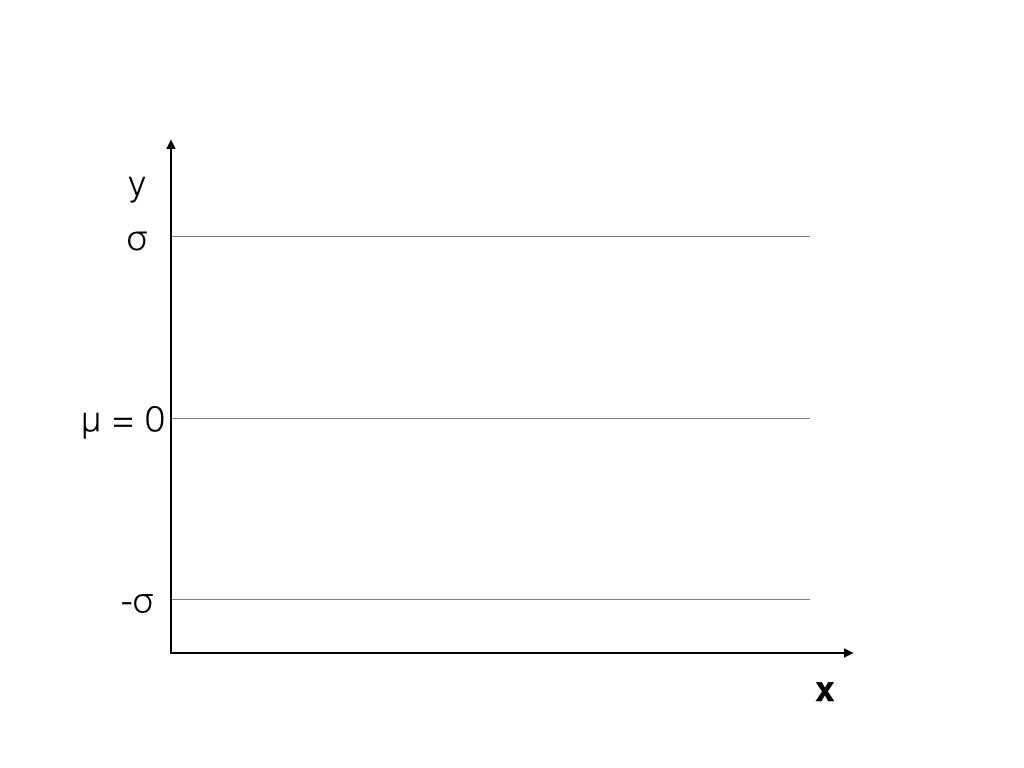
\includegraphics[width=\linewidth]{figures/GP_1.png}
  \caption{Prior with zero mean}
  \label{fig:sub1}
\end{minipage}%
\begin{minipage}{.5\linewidth}
  \centering
  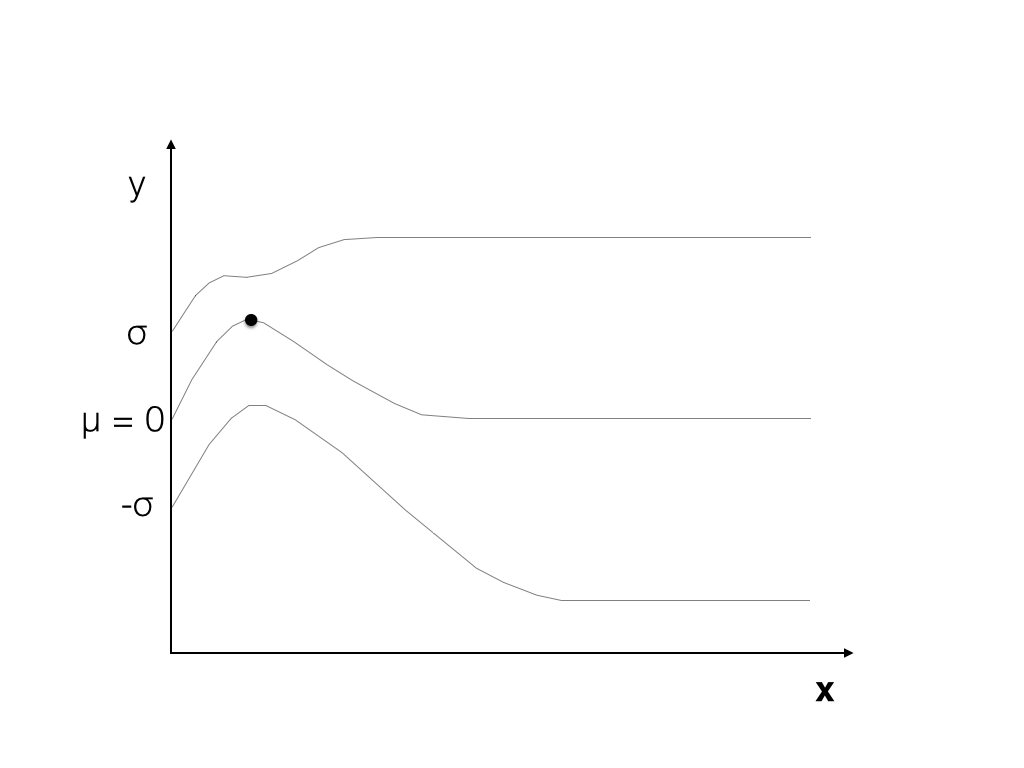
\includegraphics[width=\linewidth]{figures/GP_2.png}
  \caption{Posterior with one evidence}
  \label{fig:sub2}
\end{minipage}

\begin{minipage}{.5\linewidth}
  \centering
  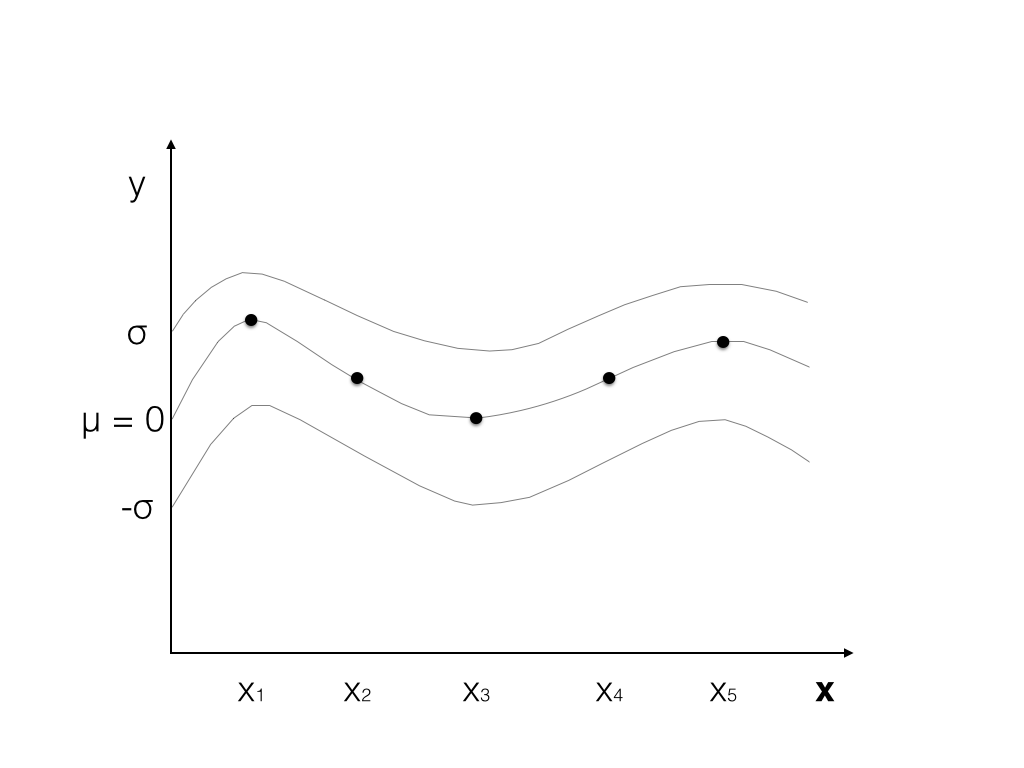
\includegraphics[width=\linewidth]{figures/GP_3.png}
  \caption{More evidences}
  \label{fig:sub1}
\end{minipage}%
\begin{minipage}{.5\linewidth}
  \centering
  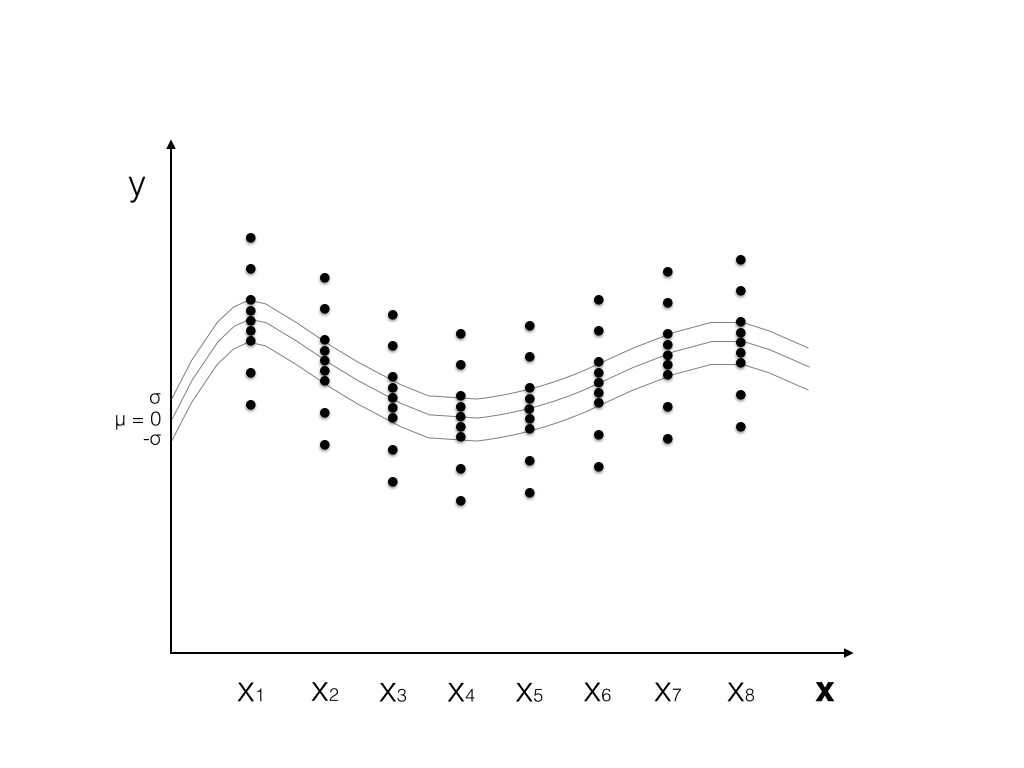
\includegraphics[width=\linewidth]{figures/GP_4.png}
  \caption{Learned function with entire training set}
  \label{fig:sub2}
\end{minipage}

\label{fig:test}
\end{figure}

We take $\mathcal{F} = \{f_1, f_2, ..., f_n, f_{n+1}, ... \infty\}$ a set of functions that can operate over $\mathbf{x}_i$. A function $f_1$ can take any form like $f_1(x) = (x + 2)$ or $f_1(x) = x^2$ or $f_1(x) = \exp(\sin(x)^5)$, as long as $f_1(x) \in \mathcal{R}$. From this infinite set $\mathcal{F}$ we need to find the proper $f$ that truly represents $y$.

To differentiate a function from a regular random variable we denote a function $f$ as $f(.)$ from now on. We start with a prior distribution over $\mathcal{F}$, given by,

\begin{equation}
f(.) \sim (m(.), k(.,.))
\end{equation}

The prior is shown in Figure 1 with zero mean. Before getting evidences, the prior distribution has uniform confidence interval around the mean for the entire space. Figure 2 shows that after getting one evidence point the space around that point shrinked. We exclude all the functions that do not pass through our evidence point. The mean function has to pass through that point, therefore it shifted and the confidence interval also narrowed down accordingly. Figure 3 shows the same effect for more evidence points. Figure 4 finally shows the shape of the posterior function when we have enough evidences.

As we are operating on a distribution over functions, the mean $m(.)$ and covariance matrix $k(.,.)$ are also functions. The domain of $f(.)$ is a vector $x_i \in \mathcal{R}^M$ where $M \to \infty$. $m(.)$ is the mean function which gives the mean of any random variable $x_{ip} (x_{ip} \in \mathbf{x}_i, p \in M)$,

$$
m(x_{ip}) = \mu_{ip}
$$

$k(.,.)$ takes two random variables, $x_{ip}$ and $x_{iq}$ and gives the covariance between them as,

$$
k(x_{ip}, x_{iq}) = Covariance(x_{ip}, x_{ip})
$$

$k(.,.)$ is also called the Kernel function.

To represent the multivariate distribution over functions operating over any finite subset $\mathbf{x}_i^m \in \mathbf{x}_i$ we can write in matrix form as,

$$
\begin{pmatrix}
f(x_1) \\
f(x_2) \\
\vdots \\
f(x_m)
\end{pmatrix}
\sim\left(%
\begin{pmatrix}
m(x_1) \\
m(x_2) \\
\vdots \\
m(x_m)
\end{pmatrix}
,%
\begin{pmatrix}
k(x_1, x_1) k(x_1, x_2) \hdots k(x_1, x_m) \\
k(x_2, x_1) k(x_2, x_2) \hdots k(x_2, x_m) \\
\vdots \\
k(x_m, x_1) k(x_m, x_2) \hdots k(x_m, x_m) 
\end{pmatrix}\right)
$$

Which can be written as,

\begin{equation}
f(\mathbf{x}_m) \sim (m(\mathbf{x}_m), K(\mathbf{x}_m))
\end{equation}

We see how easy Gaussian process is to customize, any time we can extract a finite subset out of the infinite distribution.

To simplify the calculation, we start with a zero mean prior as,

\begin{equation}
f(.) \sim (0, k(.,.))
\end{equation}

Combining Eqn. 18 and Eqn. 19 we get,

\begin{equation}
f(\mathbf{x}_m) \sim (0, K(\mathbf{x}_m))
\end{equation}

We take $\mathbf{x}_m$ as training set, so we have observed $\mathbf{y}_m$. Say we have another finite subset $\mathbf{x}_m^*$, which is the test set. We need to predict outputs $\mathbf{y}_m^*$ for $\mathbf{x}_m^*$. Both the subsets came from the same infinite Gaussian distribution. So for $\mathbf{x}_m^*$ we write,

\begin{equation}
f(\mathbf{x}_m^*) \sim (0, K(\mathbf{x}_m^*))
\end{equation}

We combine Eqn. 20 and Eqn. 21 together as,

\begin{equation}
\begin{pmatrix}
f(\mathbf{x}_m) \\
f(\mathbf{x}_m^*)
\end{pmatrix}
\sim \left( %
0, %
\begin{pmatrix}
K(\mathbf{x}_m, \mathbf{x}_m) & K(\mathbf{x}_m, \mathbf{x}_m^*) \\
K(\mathbf{x}_m^*, \mathbf{x}_m) & K(\mathbf{x}_m^*, \mathbf{x}_m^*)
\end{pmatrix}\right)
\end{equation}

We also have noise vectors $\mathbf{\varepsilon} \in \mathcal{R}^m$ and $\mathbf{\varepsilon^*} \in \mathcal{R}^m$. We get the distribution over $\mathbf{y}$ by adding noise to the distribution over $f(.)$. Addition of multiple Gaussians remains Gaussian, so we can write,

\begin{eqnarray}
\begin{pmatrix}
\mathbf{y}_m \\
\mathbf{y}_m^*
\end{pmatrix}
= %
\begin{pmatrix}
f(\mathbf{x}_m) \\
f(\mathbf{x}_m^*)
\end{pmatrix}
+%
\begin{pmatrix}
\mathbf{\varepsilon} \\
\mathbf{\varepsilon^*}
\end{pmatrix}
\sim \left( %
0, %
\begin{pmatrix}
K(\mathbf{x}_m, \mathbf{x}_m) + \sigma^2 \mathbf{I} & K(\mathbf{x}_m, \mathbf{x}_m^*) \\
K(\mathbf{x}_m^*, \mathbf{x}_m) & K(\mathbf{x}_m^*, \mathbf{x}_m^*) + \sigma^2 \mathbf{I}
\end{pmatrix}\right) \nonumber \\
\left.
\begin{pmatrix}
\mathbf{y} \\
\mathbf{y}^*
\end{pmatrix}
\right\vert_{\mathbf{x}_m, \mathbf{x}_m^*}
= %
\begin{pmatrix}
f(.) \\
f(.)^*
\end{pmatrix}
+%
\begin{pmatrix}
\mathbf{\varepsilon} \\
\mathbf{\varepsilon^*}
\end{pmatrix}
\sim \left( %
0, %
\begin{pmatrix}
K(\mathbf{x}_m, \mathbf{x}_m) + \sigma^2 \mathbf{I} & K(\mathbf{x}_m, \mathbf{x}_m^*) \\
K(\mathbf{x}_m^*, \mathbf{x}_m) & K(\mathbf{x}_m^*, \mathbf{x}_m^*) + \sigma^2 \mathbf{I}
\end{pmatrix}\right)
\end{eqnarray}

Using Bayesian posterior calculation it can be shown that,

\begin{equation}
\mathbf{y_m}^* | \mathbf{y_m}, \mathbf{x}_m, \mathbf{x}_m^* \sim (\mu^*, \Sigma^*)
\end{equation}

This is the function represented by Figure 4.

where,

\begin{equation}
\mu^* = K(\mathbf{x}_m^*, \mathbf{x}_m)(K(\mathbf{x}_m, \mathbf{x}_m) + \sigma^2 \mathbf{I})^{-1}\mathbf{y_m}
\end{equation}

and,

\begin{equation}
\Sigma^* = K(\mathbf{x}_m^*, \mathbf{x}_m^*) + \sigma^2 \mathbf{I} - K(\mathbf{x}_m^*, \mathbf{x}_m)(K(\mathbf{x}_m, \mathbf{x}_m) + \sigma^2 \mathbf{I})^{-1} K(\mathbf{x}_m, \mathbf{x}_m^*)
\end{equation}

\subsection{Upper Confidence Bound}

...

\subsection{Bandit Algorithms}

...

\subsubsection{Multi-Armed bandit}

...

\subsubsection{Contextual Bandit}

...

\subsection{Neural Networks}

...

\subsubsection{Multi-Layered Neural Network}

...

\section{Dissecting an Image}

...

\subsection{Extract objects from an Image}

...

\subsection{Extract color from an image}

...

\subsection{Combining objects and color features}

...

\section{CPU vs GPU}

...


\subsection{Why CPU is not enough}

...


\subsection{How does GPU help}

...


\section{Programming architecture of GPU}

...


\section{System design}

...

\subsection{On CPU}

...


\subsection{On GPU}

...


\section{Experiments and Results}

...


\subsection{System setup}

...


\subsection{Experiments}

...


\subsection{Performance evaluation on CPU}

...

\subsection{Performance evaluation On GPU}

...

\subsection{Performance comparison on CPU and GPU}

...


\section{User Interaction and Usability}

Design Principles -

Gestalt Laws

Norman's principles

Shneiderman's Golden Rules

Evaluation Techniques -

GOMS

KLM

Fitts Law




\nocite{*}
\bibliographystyle{tktl}
\bibliography{lahteet}

\lastpage

\appendices

\pagestyle{empty}

\internalappendix{1}{Model ABC}

The appendices here are just models of the table of contents and the presentation. Each appendix 
usually starts on its own page, with the name and number of the appendix at the top. Each appendix is paginated separately.

In addition to complementing the main document, each appendix is also its own, independent entity. 
This means that an appendix cannot be just an image or a piece of programming, but the appendix must explain its contents and meaning.


\end{document}


